\chapter{\MakeUppercase{Project implementation}}

\paragraph{} This chapter describes the implementation of the adaptive gameplay system, organized by its constituent modules and files. Each file's function, structure, and main functionality are discussed.

\section{Code Architecture Patterns}
\paragraph{} The software engineering governing the implementation of the adaptive engine strictly observes several established software design patterns to ensure robust modularity and thread-safe scalability. The primary gameplay execution wrapper implements the \textbf{Singleton Pattern}. This fundamental design choice guarantees that only a single active instance of the primary Game Engine runs in operational memory at any given time, thereby completely preventing nasty threading conflicts when the independent PyTorch subprocess attempts to read memory registers for state extraction.
\paragraph{} Furthermore, to manage the enormous, uninterrupted influx of telemetry data cleanly, the \textbf{Observer Pattern} is utilized extensively within the codebase architecture. The FastAPI telemetry dispatcher effectively acts as an isolated observer constantly monitoring the internal state variables of the \texttt{Player} class. Instead of forcing the \texttt{Player} class to redundantly write to I/O log files---action which would disastrously halt immediate movement processing every time the player takes damage---it simply broadcasts a non-blocking "State\_Changed" event. The asynchronous dispatcher thread intercepts this broadcast, packages the raw numerical state into the predefined JSON schema, and securely resolves the HTTP request back to the server. This strict and elegant structural decoupling ensures perfectly that even if the FastAPI backend unexpectedly crashes or hangs, the core space shooter game continues rendering flawlessly for the end-user.

\section{Game Module -- \texttt{game\_3d.py}}
\paragraph{} The file \texttt{game\_3d.py} is the main entry point to the game. It includes the complete game logic for the space shooter and the \ac{ai} inference pipeline for real-time difficulty adjustment. The key implementation aspects include:

\begin{itemize}
	\item \textbf{Game Initialization:} Initializes the game settings and starts the Pygame window, loads all images (for the player spaceship, enemy ships, asteroids, and projectiles), and initializes game state variables such as score, player health, and difficulty parameters.
	\item \textbf{Player Controls:} Uses keyboard inputs where WASD or Arrow keys control spaceship movement and Spacebar works for shooting. The player's position is kept within the bounds of the gaming screen.
	\item \textbf{Enemy System:} Spawns enemy ships at intervals determined by the current \texttt{spawn\_delay} parameter. Each enemy ship has health and speed attributes controlled by the \ac{dda} system. Enemies fire projectiles toward the player with frequency governed by the \texttt{attack\_intensity} parameter.
	\item \textbf{Asteroid System:} Randomly spawns asteroid objects that travel across the game field. If the player hits an asteroid, the game ends in an instant game over state.
	\item \textbf{Collision Detection:} Implements rectangle-based collision detection between player projectiles and enemies, enemy projectiles and the player, and asteroids and the player.
	\item \textbf{AI Inference Integration:} Loads the trained \ac{ppo} model from \texttt{dda\_ppo\_3d.pth} on startup. At periodic intervals during play, current player performance metrics are gathered, formatted into an observation vector, and fed into the model. The model output actions are mapped to changes in enemy speed, enemy health, spawn delay, and attack strength.
	\item \textbf{Performance Metrics Collection:} Measures accuracy ratio (shots hit / shots fired) on an ongoing basis, kill rate (enemies destroyed per unit time), player health as a percentage, damage rate (damage taken per unit time), and cumulative survival time.
\end{itemize}

\begin{figure}[!ht]
	\centering
	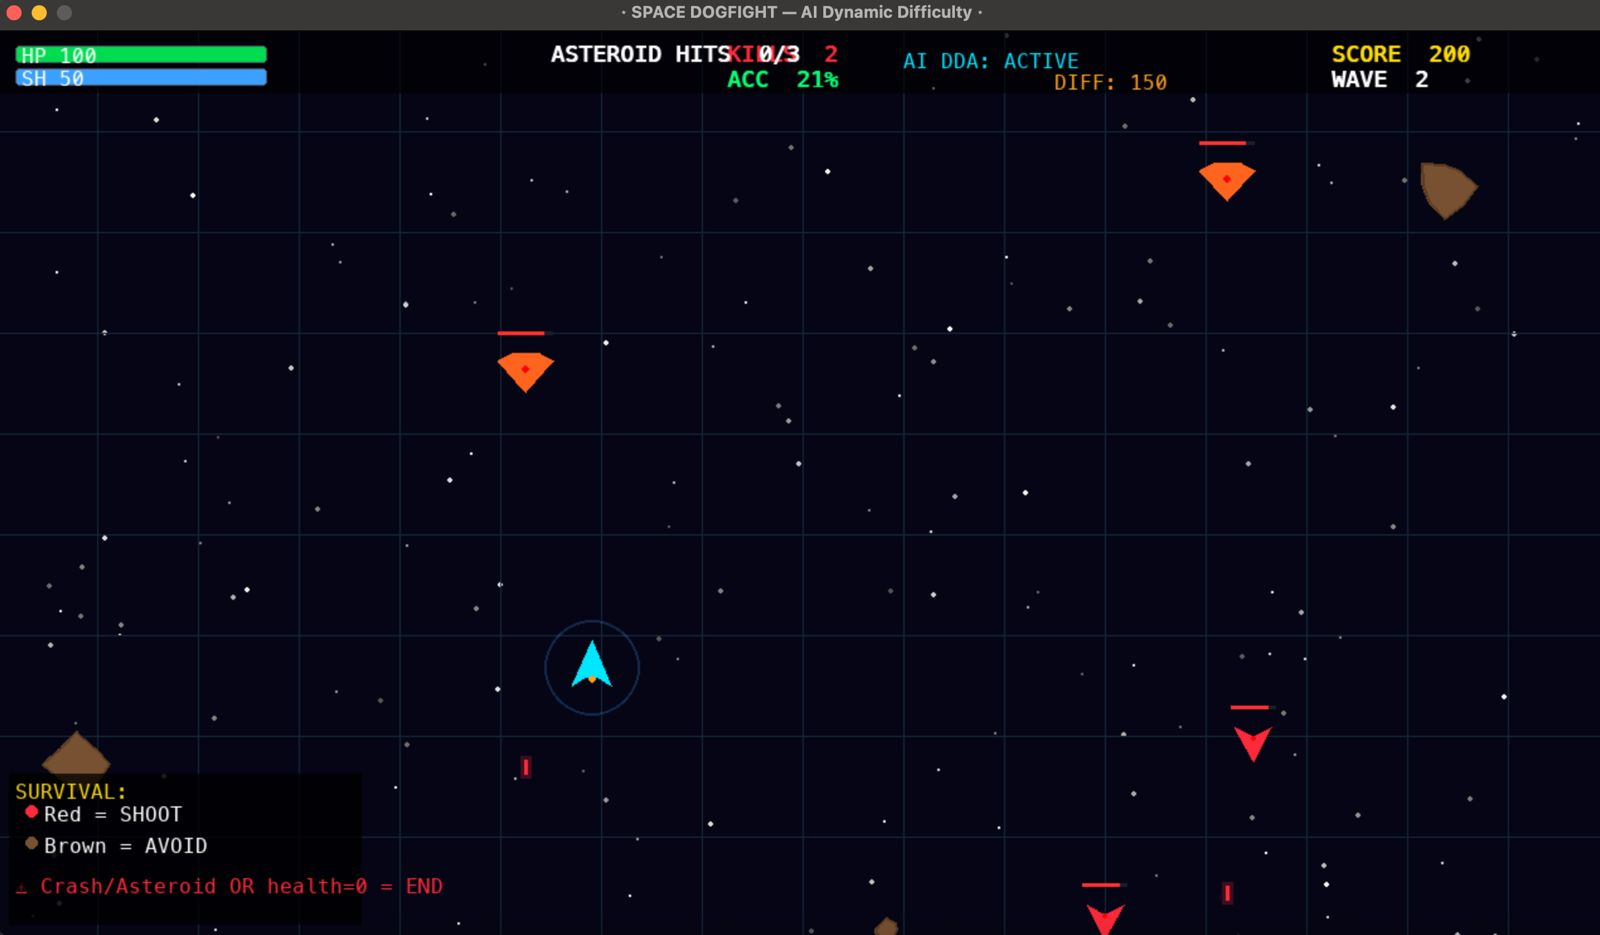
\includegraphics[width=0.9\linewidth]{images/gameplay_screenshot.png}
	\caption{In-game screenshot of the space shooter, with the player spaceship, enemy ships, projectiles, and real-time heads-up display showing health, score, and difficulty level}
	\label{fig:gameplay}
\end{figure}

\section{RL Environment -- \texttt{env\_wrapper\_3d.py}}
\paragraph{} The file \texttt{env\_wrapper\_3d.py} is the implementation of the \ac{rl} environment simulation, providing a Gymnasium-compatible interface for training the \ac{ppo} agent. Major implementation details include:

\begin{itemize}
	\item \textbf{Environment Wrapping:} Wraps the game logic in a standard \ac{rl} environment with well-defined \texttt{reset()}, \texttt{step()}, and \texttt{render()} methods.
	\item \textbf{Observation Space Definition:} Defines a continuous observation space as a seven-dimensional vector: $[\text{accuracy\_ratio}, \text{kill\_rate}, \text{dmg\_rate}, \text{health\_ratio}, \text{shield\_ratio}, \text{wave\_norm}, \text{enemies\_norm}]$, each normalized to $[0, 1]$.
	\item \textbf{Action Space Definition:} Uses a discrete action space with five actions (0--4) controlling the number of enemies and modifying the speed of the enemies.
	\item \textbf{Reward Computation:} Computes the reward function that determines how well the current difficulty settings keep the player within the engagement flow zone.
	\item \textbf{State Transition Simulation:} Approximates how players might respond to difficulty changes, enabling the agent to train without the presence of a human player during the training phase.
\end{itemize}

\section{Training Pipeline -- \texttt{train\_dda\_3d.py}}
\paragraph{} The file \texttt{train\_dda\_3d.py} implements the \ac{ppo} training pipeline using PyTorch. The key implementation components are:

\begin{itemize}
	\item \textbf{Policy Network (MLPPolicy3D):} A shared \ac{mlp} backbone with input dimension 7 (matching the observation space), three hidden layers of sizes 256, 256, and 128 with Tanh activation functions. The backbone feeds into two output heads: an actor head which produces logits over 5 discrete actions, and a critic head which outputs a scalar state value estimate $V(s)$.
	\item \textbf{Shared Architecture:} As opposed to separate actor-critic designs, the actor and critic share the feature extraction backbone, with only the final output layers being separate. This design effectively reduces the total number of parameters and enables shared representation learning.
	\item \textbf{Training Loop:} Iterates over collecting experience trajectories from the environment, computes Generalized Advantage Estimation (GAE), and updates both the policy and value networks using the \ac{ppo} clipped surrogate objective.
	\item \textbf{Hyperparameter Configuration:} Sets the learning rate ($\alpha$), discount factor ($\gamma$), clipping parameter ($\epsilon$), entropy coefficient ($\beta$), number of epochs, batch size, and rollout length.
	\item \textbf{Model Saving:} Saves the trained model weights as \texttt{dda\_ppo\_3d.pth} upon completion of training.
\end{itemize}

\subsection{Code Listings: Core PPO Neural Architecture}
\paragraph{} To clearly demonstrate the implementation level mechanics, the core PyTorch neural network definition is provided below. This highlights the shared computational backbone geometry bridging the Actor and Critic decision heads.

\begin{verbatim}
import torch
import torch.nn as nn

class SharedMLPPolicy(nn.Module):
    def __init__(self, obs_dim=7, action_space=5):
        super(SharedMLPPolicy, self).__init__()
        # Shared Feature Extractor Backbone
        self.backbone = nn.Sequential(
            nn.Linear(obs_dim, 256),
            nn.Tanh(),
            nn.Linear(256, 256),
            nn.Tanh(),
            nn.Linear(256, 128),
            nn.Tanh()
        )
        
        # Actor Head (Outputs Discrete Action Logits)
        self.actor = nn.Linear(128, action_space)
        
        # Critic Head (Outputs State Value Estimate V(s))
        self.critic = nn.Linear(128, 1)

    def forward(self, x):
        features = self.backbone(x)
        action_logits = self.actor(features)
        state_value = self.critic(features)
        return action_logits, state_value
\end{verbatim}

\paragraph{} This strict structural pattern provides extreme computational efficiency because the mathematically complex feature-extraction (the wide 256-node hidden layers) is calculated exactly once per game inference frame. The resulting optimized tensor maps are simply forwarded instantly to both specialized decision heads simultaneously, shaving precious milliseconds off the total render loop latency.

\section{Temporal Learning Extension -- \texttt{train\_dda\_3d\_lstm.py}}
\paragraph{} The file \texttt{train\_dda\_3d\_lstm.py} builds on the base training pipeline by adding \ac{lstm} layers to the policy network. This extension allows the agent to take into account a sequence of historical player performance observations instead of making decisions based on a static snapshot only. The \ac{lstm}-based architecture is particularly useful for detecting temporal trends, such as players gradually improving or declining in performance.

\subsection{LSTM Technical Integration}
\paragraph{} To mathematically and programmatically support recurrent structures, the base standard Multi-Layer Perceptron was dramatically reconfigured. Standard initial MLPs accept a rigid 1D tensor shape calculated as $[Batch, Features]$. The \ac{lstm} network, conversely, strictly requires a 3D sequential tensor shaped precisely as $[Batch, Sequence\_Length, Features]$. To securely facilitate this translation without breaking the live Pygame integration wrapper, a synchronized sliding window memory buffer of size $N=10$ was explicitly implemented. During every inference cycle, the \ac{dda} system does not uniquely send just the current isolated observation vector; instead, it sends a cohesive, chronologically ordered timeline containing the exact telemetry history of the last 10 full seconds of gameplay.
\paragraph{} The internal PyTorch architecture unwinds this sequence sequentially. The initial \ac{lstm} recurrent layers possess hidden state calculation arrays ($h_t$) and dedicated cell state memory arrays ($c_t$) that actively decode and interpret complex temporal behavioral shifts. If a player was previously playing reasonably well (resulting in a high $h_{t-1}$) but suddenly begins taking massive, repeated damage within the latest temporal sequence frames, the 'forget gate' of the \ac{lstm} aggressively flushes out the previous "optimistic" historical bias and rapidly cascades a negative severity output signal. This sequential architectural redesign effectively gives the artificial \ac{dda} neural network authentic "short-term memory," allowing for far more nuanced and human-like difficulty curves compared to standard reactionary, memory-less algorithmic baseline models.

\section{Trained Model -- \texttt{dda\_ppo\_3d.pth}}
\paragraph{} The file \texttt{dda\_ppo\_3d.pth} contains the weights of the trained \ac{ppo} model in serialized form. This file is produced by the training pipeline and is loaded by \texttt{game\_3d.py} during live gameplay. The model keeps the learned policy network parameters ($\theta$), which map player performance observations to difficulty adjustment actions.

\section{Backend API -- \texttt{backend\_fastapi}}
\paragraph{} The \texttt{backend\_fastapi} directory contains the FastAPI-based backend server implementation. Key aspects include:

\begin{itemize}
	\item \textbf{API Endpoints:} \ac{rest}ful endpoints for transmitting game session data, querying historical performance data, and providing aggregated analytics to the frontend.
	\item \textbf{Data Models:} Pydantic models that represent the gameplay log schema, including session identifiers, timestamps, player metrics, and difficulty parameters.
	\item \textbf{Session Management:} Keeps track of multiple gameplay sessions, storing and retrieving data for each player session independently.
	\item \textbf{CORS Configuration:} Set up to enable cross-origin requests from the React dashboard frontend.
\end{itemize}

\begin{figure}[h!]
	\centering
	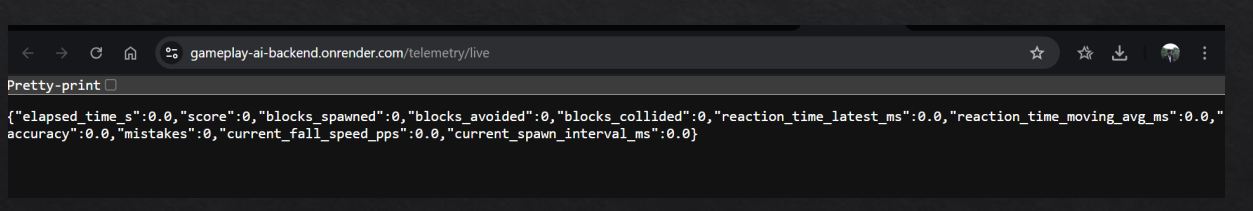
\includegraphics[width=0.9\linewidth]{images/backend_api_screenshot.png}
	\caption{FastAPI \texttt{/telemetry/live} endpoint returning real-time JSON telemetry data including elapsed time, score, accuracy, mistakes, and current difficulty parameters}
	\label{fig:backend_api}
\end{figure}

\section{Analytics Dashboard -- \texttt{dashboard}}
\paragraph{} The \texttt{dashboard} directory contains the React-based frontend application. Key features include:

\begin{itemize}
	\item \textbf{Real-Time Charts:} Interactive charts displaying player performance metrics (accuracy, kill rate, health, damage rate) over time during the course of a game session.
	\item \textbf{Difficulty Trend Visualization:} Graphs showing how difficulty parameters (enemy speed, health, spawn delay, attack intensity) change throughout a gameplay session.
	\item \textbf{Session Summary:} Overview panels displaying session-level statistics including total score, survival time, and average difficulty level.
	\item \textbf{API Integration:} Pulls data from the FastAPI backend at regular intervals to update visualizations in near real time.
\end{itemize}

\section{Analytics Tools}
\paragraph{} Three supporting modules provide additional analytics capabilities:

\begin{itemize}
	\item \textbf{\texttt{dda\_logger.py}:} Handles structured logging of gameplay events, recording player actions, difficulty adjustments, and system events to log files for post-session analysis.
	\item \textbf{\texttt{dda\_plot.py}:} Provides plotting utilities using Matplotlib to generate static visualizations of training progress, reward curves, and difficulty parameter distributions.
	\item \textbf{\texttt{dda\_curve\_visualizer.py}:} An advanced visualization tool that generates difficulty curve plots showing how the \ac{dda} system modulates game parameters over the course of a gameplay session, useful for analyzing the agent's learned behavior.
\end{itemize}
